\documentclass{article}

\usepackage{fancyhdr}
\usepackage{extramarks}
\usepackage{amsmath}
\usepackage{amsthm}
\usepackage{amsfonts}
\usepackage{tikz}
\usepackage[plain]{algorithm}
\usepackage{algpseudocode}
\usepackage{enumerate}
\usepackage{amsmath}
\usepackage{amssymb}
\usetikzlibrary{automata,positioning}

%
% Basic Document Settings
%

\topmargin=-0.45in
\evensidemargin=0in
\oddsidemargin=0in
\textwidth=6.5in
\textheight=9.0in
\headsep=0.25in

\linespread{1.1}

\pagestyle{fancy}
\lhead{\hmwkAuthorName}
\chead{\hmwkClass\ (\hmwkClassInstructor\ \hmwkClassTime): \hmwkTitle}
\rhead{\firstxmark}
\lfoot{\lastxmark}
\cfoot{\thepage}

\renewcommand\headrulewidth{0.4pt}
\renewcommand\footrulewidth{0.4pt}

\setlength\parindent{0pt}

%
% Create Problem Sections
%

\newcommand{\enterProblemHeader}[1]{
    \nobreak\extramarks{}{Problem \arabic{#1} continued on next page\ldots}\nobreak{}
    \nobreak\extramarks{Problem \arabic{#1} (cont.)}{Problem \arabic{#1} continued on next page\ldots}\nobreak{}
}

\newcommand{\exitProblemHeader}[1]{
    \nobreak\extramarks{Problem \arabic{#1} (cont.)}{Problem \arabic{#1} continued on next page\ldots}\nobreak{}
    \stepcounter{#1}
    \nobreak\extramarks{Problem \arabic{#1}}{}\nobreak{}
}

\setcounter{secnumdepth}{0}
\newcounter{partCounter}
\newcounter{homeworkProblemCounter}
\setcounter{homeworkProblemCounter}{1}
\nobreak\extramarks{Problem \arabic{homeworkProblemCounter}}{}\nobreak{}

%
% Homework Problem Environment
%
% This environment takes an optional argument. When given, it will adjust the
% problem counter. This is useful for when the problems given for your
% assignment aren't sequential. See the last 3 problems of this template for an
% example.
%
\newenvironment{homeworkProblem}[1][-1]{
    \ifnum#1>0
        \setcounter{homeworkProblemCounter}{#1}
    \fi
    \section{Problem \arabic{homeworkProblemCounter}}
    \setcounter{partCounter}{1}
    \enterProblemHeader{homeworkProblemCounter}
}{
    \exitProblemHeader{homeworkProblemCounter}
}

%
% Homework Details
%   - Title
%   - Due date
%   - Class
%   - Section/Time
%   - Instructor
%   - Author
%

\newcommand{\hmwkTitle}{Tutorial Week 11\&12}
\newcommand{\hmwkDueDate}{April 8, 2021}
\newcommand{\hmwkClass}{CZ4041}
\newcommand{\hmwkClassTime}{CS4}
\newcommand{\hmwkClassInstructor}{Assoc Prof Pan, Sinno Jialin}
\newcommand{\hmwkAuthorName}{\textbf{Pang Yu Shao}}
\newcommand{\hmwkAuthorID}{\textbf{U1721680D}}

%
% Title Page
%

\title{
    \vspace{2in}
    \textmd{\textbf{\hmwkClass:\ \hmwkTitle}}\\
    \normalsize\vspace{0.1in}\small{Due\ on\ \hmwkDueDate\ at 8:30am}\\
    \vspace{0.1in}\large{\textit{\hmwkClassInstructor\ - \hmwkClassTime}}
    \vspace{3in}\\
    \hmwkAuthorName\\
    \hmwkAuthorID
}

\date{08/04/2021}

\renewcommand{\part}[1]{\textbf{\large Part \Alph{partCounter}}\stepcounter{partCounter}\\}

%
% Various Helper Commands
%

% Useful for algorithms
\newcommand{\alg}[1]{\textsc{\bfseries \footnotesize #1}}

% For derivatives
\newcommand{\deriv}[1]{\frac{\mathrm{d}}{\mathrm{d}x} (#1)}

% For partial derivatives
\newcommand{\pderiv}[2]{\frac{\partial}{\partial #1} (#2)}

% Integral dx
\newcommand{\dx}{\mathrm{d}x}

% Alias for the Solution section header
\newcommand{\solution}{\textbf{\large Solution}}

% Probability commands: Expectation, Variance, Covariance, Bias
\newcommand{\E}{\mathrm{E}}
\newcommand{\Var}{\mathrm{Var}}
\newcommand{\Cov}{\mathrm{Cov}}
\newcommand{\Bias}{\mathrm{Bias}}

\begin{document}

\maketitle

\pagebreak

\begin{homeworkProblem}
    Suppose a dataset of four 3-dimensional instances is shown in Table 1. 
    Estimate the sample mean and covariance matrix (unbiased).

    \begin{figure}[H]
        \begin{center}
        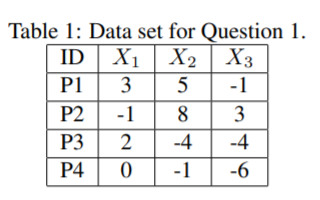
\includegraphics[scale=0.7]{resources/table1.PNG}
        \end{center}
    \end{figure}
    

    \textbf{Solution}\\
    Calculate sample mean (unbiased):
    \[
        \begin{split}
            \hat{\mu}  &= \frac{1}{N}\sum_{i=1}^{N}x_i
            \\
            &= \frac{1}{4}\begin{bmatrix}
                (3 - 1 + 2) &
                (5+8-4-1) &
                (3 - 1 - 4 - 6)
            \end{bmatrix}
            \\
            &=\begin{bmatrix}
                1 & 2 & -2
            \end{bmatrix}
        \end{split}
    \]
    Therefore, centered data matrix:\\
    \[
        \tilde{X} = \begin{bmatrix}
            2 & 3 & 1 \\
            -2 & 6 & 5 \\
            1 & -6 & -2 \\
            -1 & -3 & -4 \\
        \end{bmatrix}
    \]
    Calculate sample covariance (unbiased):
    \[
        \begin{split}
            \tilde{\Sigma}  &= \frac{1}{N-1}\sum_{i=1}^{N}(x_i - \hat{\mu})(x_i - \hat{\mu})^T
            \\
            &= \frac{1}{3}\tilde{X}^T\tilde{X}
            \\
            &=\frac{1}{3}\begin{bmatrix}
                2 & -2 & 1 & -1\\
                3 & 6 & -6 & -3\\
                1 & 5 & -2 & -4\\
            \end{bmatrix}\begin{bmatrix}
                2 & 3 & 1 \\
                -2 & 6 & 5 \\
                1 & -6 & -2 \\
                -1 & -3 & -4 \\
            \end{bmatrix}
            \\
            &= \frac{1}{3}\begin{bmatrix}
                10 & -9 & -6 \\
                -9 &  90 & 57 \\
                -6 & 57 & 46 \\
            \end{bmatrix}
            \\
            &=\begin{bmatrix}
                3.33 & -3 & -2 \\
                -3 &  30 & 19 \\
                -2 & 19 & 15.33 \\
            \end{bmatrix}
        \end{split}
    \]
    

\end{homeworkProblem}
\newpage
\begin{homeworkProblem}
    Suppose a dataset of 5 1-dimensional instances is shown in Table 2. Use histogram estimator with an origin of 0 and a width of 3,
    naive estimator with a width of 3, and 3-NN estimator to estimate the density function $\hat{p}(x)$ and compute the value of 
    $\hat{p}(2.6)$ at 2.6, respectively.

    \begin{figure}[H]
        \begin{center}
        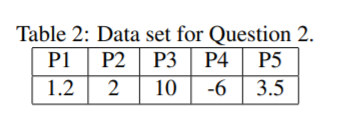
\includegraphics[scale=0.7]{resources/table2.PNG}
        \end{center}
    \end{figure}
    
    \textbf{Solution}\\
    For \textbf{histogram estimator}:\\
    Window: ${0 \leq x_i < 3}$\\
    \[
        \begin{split}
            \hat{p}(2.6) &= \frac{2}{5*3}
            \\
            &= 0.133
        \end{split}
    \]
    For \textbf{naive estimator}:\\
    Window: ${1.1 \leq x_i < 4.1}$\\
    \[
        \begin{split}
            \hat{p}(2.6) &= \frac{3}{5*3}
            \\
            &= 0.2
        \end{split}
    \]
    For \textbf{K-NN estimator}:\\
    Distance from x=2.6:\\
    
    P2: 0.6\\
    P5: 0.9\\
    \textbf{P1: 1.4 (3rd nearest neighbour)}\\
    P3: 7.4\\
    P4: 8.6\\

    \[
        \begin{split}
            \hat{p}(2.6) &= \frac{3}{5*(2*1.4)}
            \\
            &= 0.214
        \end{split}
    \]
            

\end{homeworkProblem}
\newpage
\begin{homeworkProblem}
    A dataset of five 4-dimensional instances is given in Table 1. Suppose a SVD is performed 
    on the data matrix X (5-by-4) via $X = VDU^T$, and the matrices U, D and V are shown in Tables 2-4,
    respectively. Use principal component analysis to project the 5 datapoints in Table 1 to 2-dimensional
    space.

    \begin{figure}[H]
        \begin{center}
        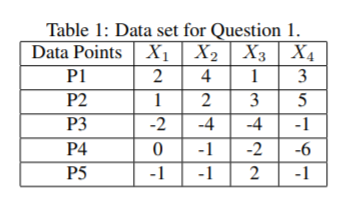
\includegraphics[scale=0.7]{resources/12a.PNG}
        \end{center}
    \end{figure}
    \begin{figure}[H]
        \begin{center}
        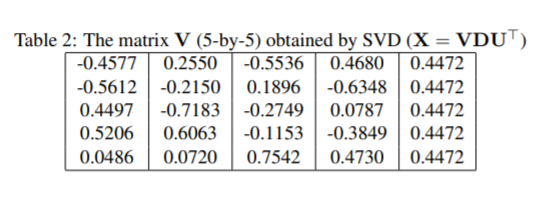
\includegraphics[scale=0.7]{resources/12b.PNG}
        \end{center}
    \end{figure}
    \begin{figure}[H]
        \begin{center}
        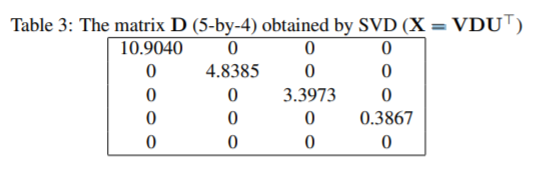
\includegraphics[scale=0.7]{resources/12c.PNG}
        \end{center}
    \end{figure}
    \begin{figure}[H]
        \begin{center}
        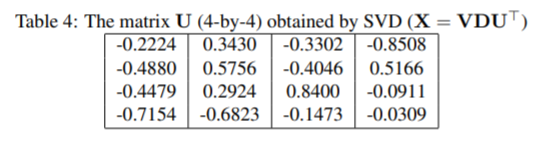
\includegraphics[scale=0.7]{resources/12d.PNG}
        \end{center}
    \end{figure}
    \newpage
    \textbf{Solution}\\
    First, we center the datapoints in X
    \[
    \begin{split}
        X &= 
        \begin{bmatrix}
            2 & 4 & 1 & 3 \\
            1 & 2 & 3 & 5 \\
            -2 & -4 & -4 & -1\\
            0 & -1 & -2 & -6\\
            -1 & -1 & 2 & -1
        \end{bmatrix}
        \\\\
        \mu &= \begin{bmatrix}
            0&0&0&0 \\
        \end{bmatrix}
        \\
    \end{split}    
    \]
    Therefore, datapoints are already centered.\\\\
    2. Calculate the covariancematrix $\tilde{\Sigma}$,
    \[
    \begin{split}
        \tilde{\Sigma} &= \frac{1}{5-1}X^TX
        \\
        &= U\tilde{D}U^T, \tilde{D} = \frac{1}{4}D^TD 
        \\
    \end{split}    
    \]
    3. Find Eigenvalues/ Eigenvectors of the Covariance matrix.\\
    Since $U^TU = I$,
    \[
    \begin{split}
        \tilde{\Sigma}U &= \tilde{D}U
        \\
        \tilde{D} &= \frac{1}{4}\begin{bmatrix}
            10.90^2 & 0 & 0 & 0 \\
            0 & 4.84^2 & 0 & 0 \\
            0 & 0 & 3.40^2 & 0\\
            0 & 0 & 0 & 0.39^2\\
        \end{bmatrix}
    \end{split}    
    \]
    Therefore, the first two columns of the U matrix correspond to the 
    top two eigenvectors with the highest eigenvalues. We select the first 2 columns
    to construct the top 2 principal components.
    \[
    \begin{split}
        XU &= \begin{bmatrix}
            2 & 4 & 1 & 3 \\
            1 & 2 & 3 & 5 \\
            -2 & -4 & -4 & -1\\
            0 & -1 & -2 & -6\\
            -1 & -1 & 2 & -1
        \end{bmatrix}
        \begin{bmatrix}
            -0.2224 & 0.3430\\
            -0.4880 & 0.5756\\
            -0.4479 & 0.2924\\
            -0.7154 & -0.6823
        \end{bmatrix}
        \\
        &=\begin{bmatrix}
            -4.99 & 1.23\\
            -6.12 & -1.04\\
            4.90 & -3.48\\
            5.68 & 2.93\\
            0.53 & 0.35
        \end{bmatrix}
    \end{split}    
    \]

    \begin{figure}[H]
        \begin{center}
        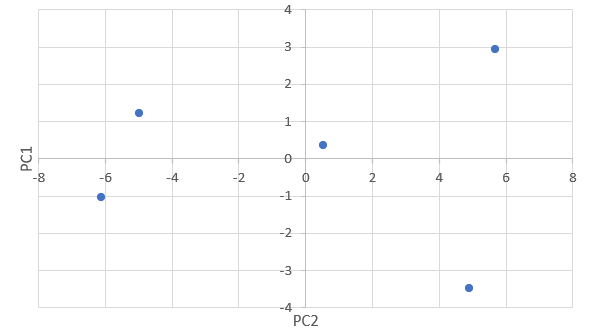
\includegraphics[scale=0.9]{resources/pca.PNG}
        \end{center}
    \end{figure}



        

\end{homeworkProblem}


\end{document}